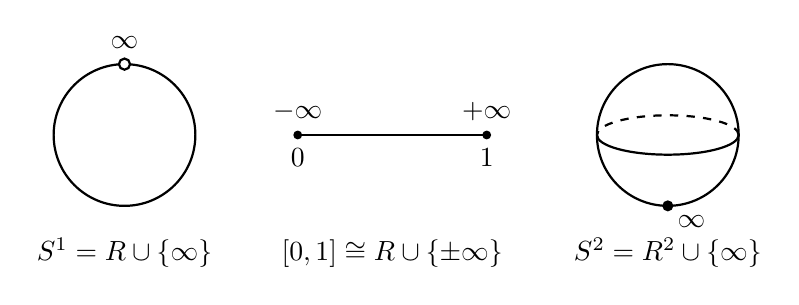
\begin{tikzpicture}[scale=1]
% (a) circle
\draw[thick] (0,0) circle (0.9);
\draw[thick, fill=white] (0,0.9) circle (2pt);
\node[above=2pt] at (0,0.9) {$\infty$};
\node at (0,-1.5) {$S^1 = \mathbb{R}\cup\{\infty\}$};
% (b) interval
\draw[thick] (2.2,0) -- (4.6,0);
\fill (2.2,0) circle (1.6pt);
\fill (4.6,0) circle (1.6pt);
\node[below] at (2.2,-0.05) {$0$};
\node[below] at (4.6,-0.05) {$1$};
\node[above] at (2.2,0.05) {$-\infty$};
\node[above] at (4.6,0.05) {$+\infty$};
\node at (3.4,-1.5) {$[0,1] \cong \mathbb{R}\cup\{\pm\infty\}$};
% (c) sphere
\draw[thick] (6.9,0) circle (0.9);
\draw[thick] (6.0,0) arc (180:360:0.9 and 0.25);
\draw[thick, dashed] (7.8,0) arc (0:180:0.9 and 0.25);
\fill (6.9,-0.9) circle (2pt);
\node[below right] at (6.9,-0.9) {$\infty$};
\node at (6.9,-1.5) {$S^2 = \mathbb{R}^2\cup\{\infty\}$};
\end{tikzpicture}
